
\exercise{Mean degree distribution}{4}
The following figure shows the probability that a network drawn from an ER ensemble with mean degree $2$ has actually a mean degree of $z$, where $z$ is not necessarily $z$,
\begin{center}
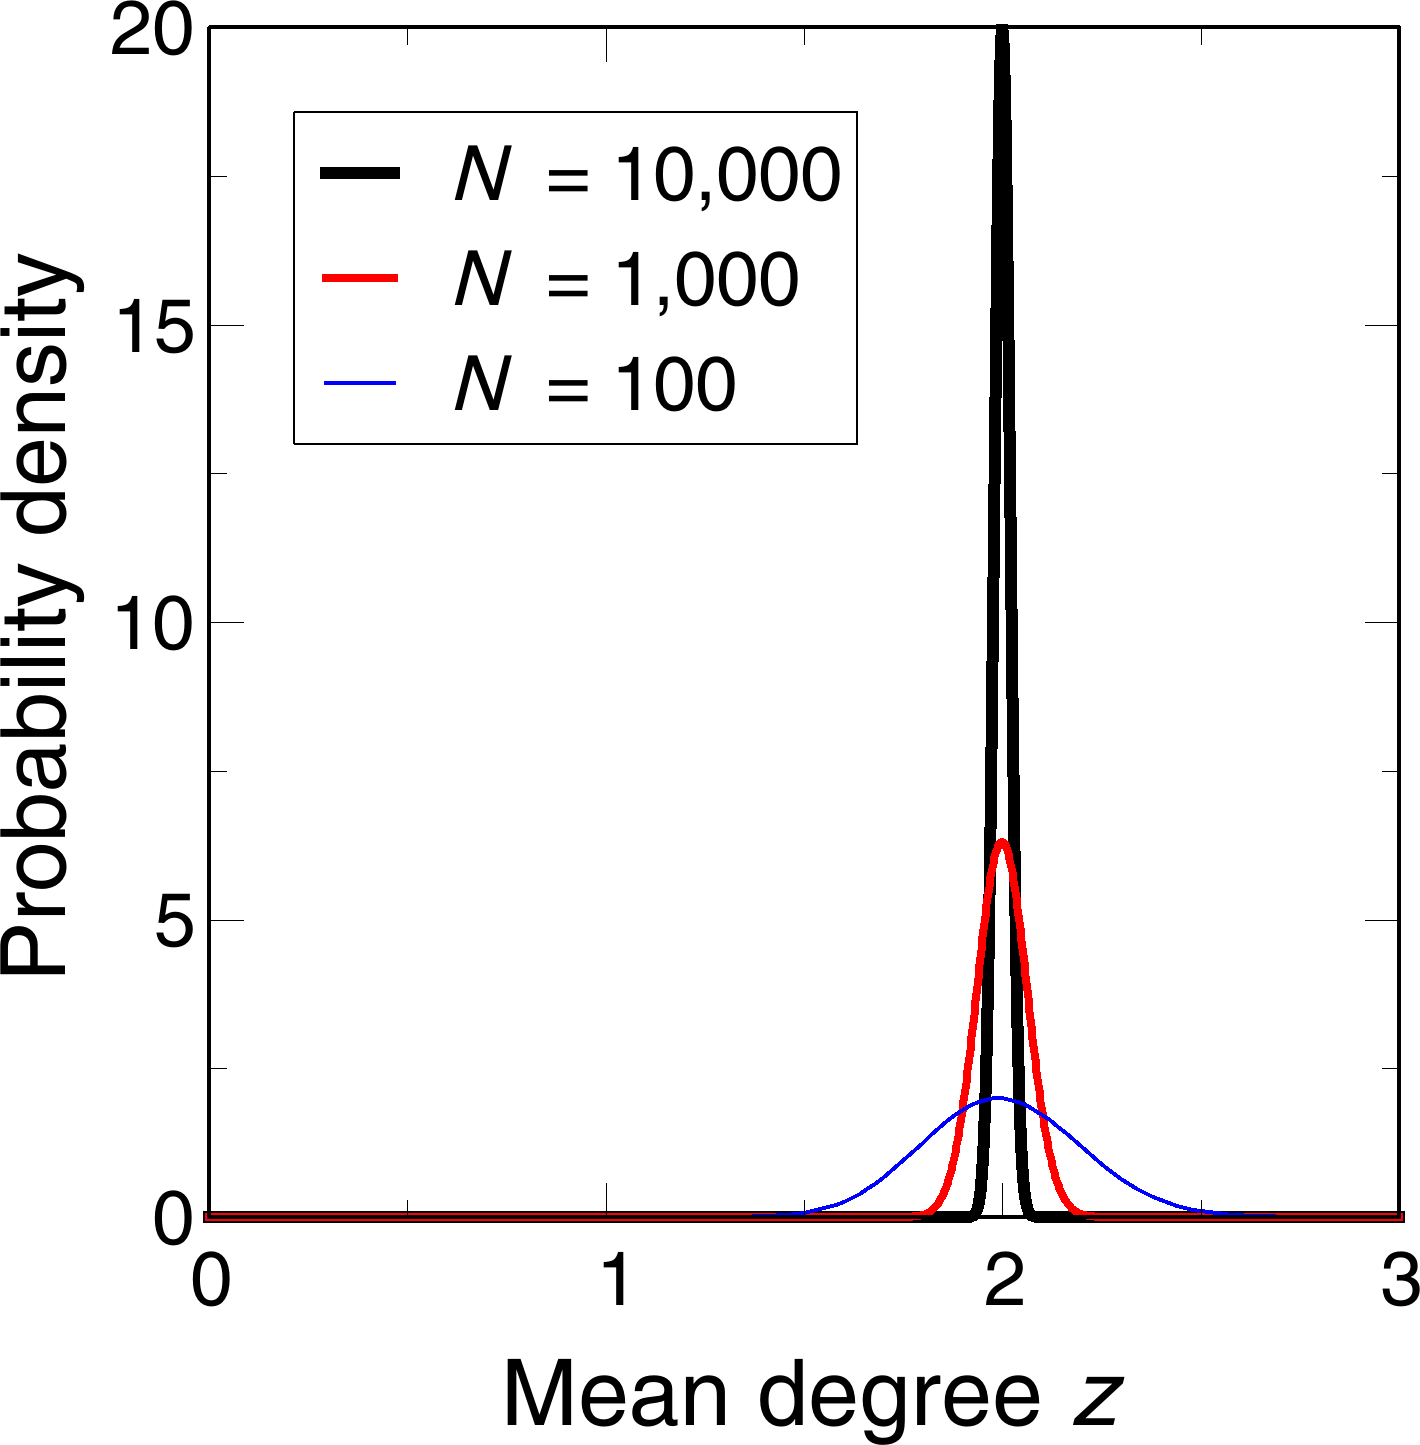
\includegraphics[width=0.4\textwidth]{netsdistribution.png}
\end{center}
But how was this figure actually made? 

\subquestion Find a way to compute the probability that a network of 100 nodes drawn from an ensemble with mean degree 2 actually has mean degree 2. 

\solution
Since we are dealing with a network of $N=100$ nodes, mean degree $z=2$ of the network requires that $K=100$ links are placed during the network creation as we know 
\eq{
z=\frac{2K}{N}.
}
The number of chances to place a link is identical to the number of distinct pairs of nodes in the network. Already from Chap.~1 we know 
\eq{
K_{\rm max} = \frac{N(N-1)}{2}.
}
This is the number of maximal links that a simple graph of this size could contain, but also the number of trials for placing links in the network creation. In our case of $N=100$ it is
\eq{
K_{\rm max} = \frac{100\cdot 99}{2} = 4950.
}
Each of these trials succeeds and places a link with probability $p$. From this chapter we know that we need to chose 
\eq{
p=\frac{z}{N-1} = \frac{2}{99}
}
to give the ensemble the desired mean degree of 2. The complementary probability of not placing a link in the trial is then 
\eq{
q= 1-p= \frac{97}{99}.
}
So the probability that a specific set of 100 links is placed and no other links is placed is 
\eq{
p^{K}q^{K_{\rm max}-K} = p^{100}q^{4850} 
}
and of course the number of ways in which we can pick the specific 100 links we want to built from the set of 4950 potential links is 
\eq{
B(K_{\rm max},K)=\frac{K_{\rm max}!}{(K_{\rm max}-K)!K!} 
}
Now putting everything together we can write the probability that a network drawn from the ensemble has $K$ links as 
\eq{
  p^{K}q^{K_{\rm max}-K} B(K_{\rm max},K) = \left(\frac{2}{99}\right)^{100}\left(\frac{97}{99}\right)^{4580}\frac{100! 4850!}{4950!} 
}
Are we done yet? No, because this equation is quite horrible. We certainly don't want to compute the factorial of 4950 and also $(2/99)^{100}$ may give you numerical trouble. So,  we need to simplify this a bit. 

Note that our equation describes a binomial distribution. 
The Poisson distribution 
\eqn{
  \frac{z^k \exp{-z}}{k!}
}
approximates the probability of drawing a result $k$ from a binomial distribution with mean $z$. In the present case we are interested in the probability of drawing $K$ from a binomial distribution where the average result is $K_*=Nz/2$ is the expected number of links in a network drawn from the distribution. Replacing the respective values yields the approximation 
\eq{
p^{K}q^{K_{\rm max}-K} B(K_{\rm max},K) \approx \frac{ {K_*}^K \exp{-K_*}}{K!}
}
Hence, we can find the answer to our question by evaluating 
\eq{
\frac{{100}^{100} \exp{-100}}{100!} \approx 0.04
}
which is a surprisingly sane result from an expression that is still a bit crazy. 

\subquestion Bonus: How does your probability relate to the probability density shown in the figure, and why does the figure show probability density, rather than probability directly? (If you are unsure check out the explanation in the solution) 

\solution

Probabilities are quite intuitive but they are not well suited when we compare distributions with different numbers of values. Consider that the figure shows the probabilities for networks up to mean degree 3. For $N=100$ nodes this means the probabilities for networks with 0 to 150 links are shown in the figure, so 151 possible outcomes in total. By contrast for $N=10000$ nodes there are 15001 possible values that can be realized in the same interval. Due to the much higher number of outcomes in the larger network each one outcome has individually a much lower probability, which makes is difficult to visualize and meaningfully compare the distribution from network of different size. 

The solution to this problem is to convert the individual probabilities into a probability density, that is in this case probability per unit of $z$. To do this conversion we only need to divide the probabilities by the average $z$-distance between out comes. For example for the network with $N=100$ two consecutive values of $z$ that are possible differ by one link. For example at $K=100$ links the network has mean degree $z=2$. The next denser network that is possible has $K=101$ links for a mean degree  of $z=2.02$ hence the distance between adjacent outcomes is $0.02$ So to convert the probabilities into probability densities we take our computed probabilities and divide them by 0.02, which is the same as multiplying them by 50. For the outcome probability density at $z=2$ in the network with $N=100$ we find $0.04\cdot 50 = 2$, which is the value shown in the figure. 

Probability densities are convenient to interpret visually as the integral over the curve should always be 1. Hence even of networks are now described by curves that have the same volume under the curve. 

